\documentclass[11pt]{article}
\usepackage[utf8]{inputenc}
\usepackage[T1]{fontenc}
\usepackage[margin=2.5cm]{geometry}
\usepackage{graphicx}
\usepackage{booktabs}
\usepackage{array}
\usepackage{amsmath}
\usepackage{amssymb}
\usepackage{listings}
\usepackage{xcolor}
\usepackage{hyperref}
\usepackage{multirow}

\lstset{
  basicstyle=\ttfamily\small,
  breaklines=true,
  columns=fullflexible,
  frame=single
}

\title{Informe}
\author{}
\date{}

\begin{document}
\maketitle

\section*{Integrantes}
\begin{itemize}
  \item Cristobal Albornoz
  \item Sebasti\'an Barr\'ia
  \item Benjam\'in Pe\~na
\end{itemize}

\section*{Respuestas incisos}

\subsection*{b) Implementaci\'on de bootstrapping}

Se cre\'o un archivo de utils compartidas \texttt{common.py} y un archivo para cada una de las implementaciones de bootstrapping:

\subsubsection*{common.py}

\begin{itemize}
  \item El ajuste lineal se resuelve por factorizaci\'on directa en vez de invertir matrices expl\'icitamente.
  \item Cada resample bootstrap se construye usando una identidad algebraica que evita reconstruir el dataset completo por repetici\'on: se trabaja con pesos y se descartan las filas no sorteadas, reduciendo el volumen de c\'omputo por tarea.
\end{itemize}

\subsubsection*{bs\_auto.py}

Delega el bootstrapping y el paralelismo por completo a una librer\'ia externa. No aplica el descarte de filas no sorteadas ni la construcci\'on optimizada del resample, por lo que hace m\'as trabajo por tarea que las otras dos versiones.

\subsubsection*{bs\_sklearn.py}

Aplica la construcci\'on optimizada del resample (pesos + descarte de filas), pero el ajuste final usa un m\'etodo num\'erico m\'as costoso propio de la librer\'ia, que es el cuello de botella de esta versi\'on.

\subsubsection*{bs\_numpy.py}

La versi\'on que m\'as se pudo optimizar: combina paralelismo expl\'icito, construcci\'on eficiente del resample y resoluci\'on directa del sistema de ecuaciones normales, minimizando tanto el trabajo por tarea como la sobrecarga de c\'omputo. Es la m\'as r\'apida en tiempo absoluto, pero por lo mismo la m\'as sensible a la sobrecarga fija de paralelizaci\'on (cada tarea es tan liviana que el costo de repartirla entre procesos pesa proporcionalmente m\'as).

\subsection*{c) Correctitud y reproducibilidad}

\subsubsection*{i)}

Respecto a los IC, a nivel general, se usa una funci\'on \textit{ci\_percentil()} para poder calcularlos de igual manera al final de la ejecuci\'on de cada una de las variantes del algoritmo, entregando los \textit{betas} calculados y el \textit{alpha=0.05}, resultando en descartar 1 valor por lado (descarta el 2.5\% superior o inferior, equivalente al multiplicar por B=48 --> 1) y lograr un nivel de confianza de 95\% aproximadamente. Para verificar esto, se utiliza la funci\'on \textit{cobertura()}, para poder calcular la fracci\'on de los coeficientes verdaderos (BETA\_STAR) que quedan dentro del IC, la cual se espera que rondee ese 95\% en los resultados emp\'iricos.

En cuanto a los resultados obtenidos, al revisar el reporte obtenido en \textit{tiempos\_XXXX.csv} con XXXX = computador en el que fueron ejecutados los algoritmos, se puede apreciar que los IC tienden a tener caracter\'isticas id\'enticas (ancho del IC promedio, cobertura de BETA\_STAR y error relativo de BETA\_STAR) para las variantes \textit{sklearn} y \textit{numpy}, y ligeramente distintas para las de la versi\'on \textit{auto} (tiene ligeramente peor cobertura, error relativo y es menos ancho que las otras 2).

Los resultados para cada una de las m\'etricas se adjuntan a continuaci\'on:

\begin{center}
\begin{tabular}{lrrr}
\toprule
M\'etrica & PC-1 (sebas) & PC-2 (kintsugi) & PC-3 (aurora-ferrum) \\
\midrule
Ancho & 0.024227 (+) & 0.011812 & 0.011812 \\
Cobertura & 88,5\% (-) & $\sim$95\% & $\sim$95\% \\
Error relativo & 0.00220527 (+) & 0.00042929 & 0.00042929 \\
\bottomrule
\end{tabular}
\end{center}

\subsubsection*{ii)}

En cuanto a equivalencia, tanto \textit{bs\_numpy} como \textit{bs\_sklearn} usan \texttt{common.child.seeds(B)} (que usa SeedSequence) y \texttt{common.bootstrap\_weights(rng, N)} bajo la misma secuencia de semillas generados por ella, lo que significa que ambas versiones sortean los mismos N \'indices para el resample \textit{b}, por ende armando los mismos $X^{(b)}$ e $y^{(b)}$ ponderado, siendo la \'unica diferencia entre ambas el algoritmo usado para resolver el \'algebra lineal del problema:
\begin{itemize}
  \item bs\_numpy: resuelve mediante ecuaciones normales con \texttt{np.linalg.solve}, que hace uso de factorizaci\'on LU en el producto de X con su transpuesta
  \item bs\_sklearn: resuelve mediante \texttt{LinearRegression}, que se basa en SVD (Descomposici\'on de Valores Singulares)
\end{itemize}
Como ambos m\'etodos resuelven el mismo sistema, las diferencias entre sus resultados probablemente se deban a errores de redondeo de puntos flotantes, lo cu\'al tiene ordenes de magnitud muy bajos ($1\times10^{10}$ o $10^{12}$ aprox), lo que se traduce en resultados casi id\'enticos, como se puede ver en las m\'etricas antes mencionadas, donde para ambos computadores dan = valores.

Por otro lado, \textit{bs\_auto} es comparable pero no tan id\'entido, de ah\'i la ligera diferencia entre valores vistos previamente, pues utiliza \texttt{BaggingRegressor} el cual hace su propio muestreo bootstrap interno con su propio generador de \'indices distntos al SeedSequence utilizado por los otros 2. As\'i, aunque se est\'e usando la misma semilla, al tener un mecanismo de generaci\'on de n\'umeros aleatorios distinto al \texttt{common.child.seeds(B)}, los \'indices que termina sorteando no coinciden resample a resample con los de \textit{bs\_numpy} y \textit{bs\_sklearn}.
\begin{itemize}
  \item Aqu\'i cabe mencionar que la diferencia radica principalmente en ese muestreo distintos del conjunto de B coeficientes, pero el mecanismo de bootstrap se mantiene el los 3, por lo que siempre es comparable
  \item Otro aspecto a considerar, aunque del lado computacional, no de resultados, es que \textit{bs\_auto} no descarta la fila de peso 0 a diferencia de la implementaci\'on en \texttt{common.weighted\_design}, lo que si las descarta, lo que lo hace m\'as lento como se puede ver en los resultados de los .csv
\end{itemize}

\subsubsection*{iii)}

Para que los resultados sean reproducibles se necesita:
\begin{itemize}
  \item \textbf{= semilla en la generaci\'on de datos}: Por ello en \texttt{gen\_data.py} se usa una semilla fija al momento de ejecutar \texttt{np.random.default\_rng(seed)} al crear los datos sint\'eticos aleatorios, lo que logra que X y BETA\_STAR sean ide\'ntidos entre ejecuciones y computadores.
\end{itemize}

\textbf{NOTA}: Adem\'as, se guardan los arreglos en un \textit{.npy} para que las 3 variantes de bootstrapping puedan usar los mismos datos y puedan mediante \textit{mmap mode="r"} poder abrirlos sin duplicar la memoria entre procesos. Esto es lo que queda en la carpeta \textbf{/data} en forma de \texttt{beta\_star.npy, X.npy, y.npy}

\begin{itemize}
  \item \textbf{semillas independientes por resample y desacopladas de p}: Como \texttt{default\_rng(seed + b)} no da garant\'ias de independencias entre streams, pudiendo haber colisiones, si se usara podr\'ia hacer que el resultado de las operaciones dependa del orden de ejecuci\'on y por ende de \textit{p}. Por ello se plantea usar \texttt{p.random.SeedSequence().spawn(B)} en \texttt{common.child\_seeds}, para generar B streams estad\'isticamente independientes (lo garantiza al alejarlos mucho mediante el uso de hashing criptogr\'afico) y generar streams que provoquen que el mismo resample \textit{b} ($b=i$) siempre reciba la misma semilla hija, sin importar cuantos procesos p se usen o c\'omo \textit{joblib} reparta las tareas entre ellos
  \begin{itemize}
    \item Esto es la base que permite comparar tiempos de ejecuci\'on para sitinto \textit{p} sin que el valor del resultado cambie
  \end{itemize}
  \item \textbf{= numero de hilos internos}: Como el producto de X con su transpuesta se calcula con BLAS y este puede llegar a usar m\'ultiples hilos, la suma de los productos internos puede hacerse en distintos orden seg\'un esos distintos hilos, afectando el resultado, por ello para lograr una reproductibilidad m\'as exacta conviene usar el mismo n\'umero de hilos internos
  \item \textbf{= versi\'on de las librer\'ias}: como la implementaci\'on depende mucho del funcionamiento de las librer\'ias (Numpy, Sklearn, ...), variaciones de versiones en estas pueden generar algoritmos ligeramente distintos, lo que puede generar cierta variabilidad aunque sea menor en los resultados, por ello conviene usar = version para lograr una buena reproductibilidad
  \item \textbf{= dtype}: La cossa cambia si uno usa puntos flotantes de tipo \textit{float32} que \textit{float64}, por ello para fomentar la reproducibilidad, conviene usar = tipo de dato
  \item \textbf{no reusar estado entre versiones/subprocesos}: as\'i evitando que el pool del backend utilizado pueda contaminar la siguiente medici\'on, por eso \texttt{bench.py} hace que cada subproceso sea una nueva versi\'on. Esto m\'as que nada respecto a reproducibilidad temporal que resultados
\end{itemize}

\subsection*{d) Backend de multiprocessing de joblib}

\subsubsection*{i)}

El backend de \textbf{multiprocessing} utiliza por defecto \textbf{loky} (adem\'as se setea \textbf{loky} a lo largo de la tarea) y gestiona la creaci\'on de los \textbf{p} procesos hijo. Para la creaci\'on de procesos normalmente se usa \textbf{fork} en Linux y \textbf{spawn} en macOS y Windows
\begin{itemize}
  \item \textbf{fork:} aqu\'i el SO clona el proceso padre, creando un proceso hijo que tiene una copia ide\'ntica del espacio de direcciones y la tabla de p\'aginas de la memoria virtual del padre
  \item \textbf{spawn:} inicia un ejecutable de Python desde 0, completamente limpio: nuevo interprete, reimporta m\'odulos y reconstruye el contexto de ejecuci\'on pasando los argumentos v\'ia serializaci\'on
\end{itemize}

En cuanto a la asignaci\'on de memoria, \textbf{fork} intenta utilizar \textbf{Copy on Write (CoW)}, evitando asignar nueva memoria RAM f\'isica, por ende duplicando los datos del programa, sino que hace que el proceso hijo comparta las mismas p\'aginas f\'isicas de la RAM que su padre bajo solo permisos de lectura. As\'i, solo cuando el padre o el hijo intenten escribir en esa p\'agina, el sistema hage un \textbf{page fault}, duplicando esa p\'agina espec\'ifica y le asigna memoria RAM f\'isica dedicada al hijo. Pero, existe el gran problema que el Garbage Collector y el contador de referencias modifican los encabezados (contadores de referencia) de los objetos en memoria constantemente, incluso para operaciones de lectura, lo que rompe la optimizaci\'on del \textbf{COW}, forzando al SO a duplicar las p\'aginas de RAM innecesariamente.
\begin{itemize}
  \item Si se utilizara \textbf{spawn}, se asigna un bloque de RAM independiente desde el inicio, por lo que eso no pasa
\end{itemize}

\subsubsection*{ii)}

En cuanto al manejo de \textbf{X} e \textbf{y} en \textit{Joblib}, para arreglos grandes de NumPy (umbral de 1 MB aprox) \textit{joblib} usa \textbf{Memory Mapping (memmap)}, almacenando termporalmente los arreglos en una RAM compartida (/dev/shm) antes de lanzar las tareas paralelas, entregando solo punteros de lectura mapeados en memoria a cada uno de los \textbf{p} procesos (no copias de los datos). As\'i los procesos leen directamente de los bloques de la matriz original de la RAM, generando un acceso concurrente sin duplicaci\'on.

Esto se hace para evitar caer en usar los pipes estandar de \textbf{multiprocessing}, en los cuales se tendr\'ia que aplicar \textbf{pickling (serializaci\'on)} a los arreglos y transmitirlos mediante los canales (sockets/pipes) de IPC (comunicaci\'on entre procesos) a cada uno de los \textbf{p} procesos, lo cual generar\'ia un consumo masivo de memoria al duplicar \textbf{p} veces los arreglos en la RAM, adem\'as de a\~nadir la penalizaci\'on temporal relacionada a la serializaci\'on

\subsection*{e) Inspecci\'on de threads}

\subsubsection*{i)}

Se corri\'o el siguiente c\'odigo en PC-3 (ver specs en inciso f). Primero con el numero exacto de cores f\'isicos:

\begin{lstlisting}[language=sh]
python bs_numpy.py -p 8
============================
[bs_numpy] p=8 B=48 hilos_internos=1 dtype=float64
  tiempo bootstrap :    1.949 s
  hilos totales    : 8 (nucleos fisicos: 8) tasa uso : 1.0
  ancho IC medio   : 0.011812
  cobertura beta*  : 0.950
  ||mean(b)-bhat|| : 4.29e-04
\end{lstlisting}

Luego, con el numero exacto de cores l\'ogicos:

\begin{lstlisting}[language=sh]
python bs_numpy.py -p 16
============================
[bs_numpy] p=16 B=48 hilos_internos=1 dtype=float64
  tiempo bootstrap :    2.476 s
  hilos totales    : 16 (nucleos fisicos: 8) tasa uso : 2.0
  ancho IC medio   : 0.011812
  cobertura beta*  : 0.950
  ||mean(b)-bhat|| : 4.29e-04
\end{lstlisting}

Y finalmente con un n\'umero mayor al de cores l\'ogicos:

\begin{lstlisting}[language=sh]
python bs_numpy.py -p 32
============================
[bs_numpy] p=32 B=48 hilos_internos=1 dtype=float64
  tiempo bootstrap :    2.672 s
  hilos totales    : 32 (nucleos fisicos: 8) tasa uso : 4.0
  ancho IC medio   : 0.011812
  cobertura beta*  : 0.950
  ||mean(b)-bhat|| : 4.29e-04
\end{lstlisting}

Notamos que luego de sobrepasar el numero de cores f\'isicos el tiempo de bootstrap toma m\'as tiempo, lo que es un s\'intoma de la sobresubscripci\'on.

\subsubsection*{ii)}

Notamos que en el c\'odigo el problema ocurre dado que no se limita el numero m\'aximo de workers seg\'un los cores f\'isicos. Por lo que se puede prevenir este problema al agregar un techo tal que:

\[
p \leq \text{cores\_fisicos}
\]

\subsection*{f) Cores l\'ogicos de computador}

\begin{center}
\begin{tabular}{lrrr}
\toprule
M\'etrica & PC-1 (sebas) & PC-2 (kintsugi) & PC-3 (aurora-ferrum) \\
\midrule
Cores l\'ogicos & 8 & 8 & 16 \\
Cores f\'isicos & 4 & 4 & 8 \\
\bottomrule
\end{tabular}
\end{center}

\subsubsection*{Resultados}

\begin{center}
\begin{tabular}{clrrr}
\toprule
PC & p & bs\_auto & bs\_numpy & bs\_sklearn \\
\midrule
\multirow{4}{*}{PC-1} & 1 & 73.493 & 6.431 & 42.273 \\
 & 2 & 71.334 & 4.848 & 41.773 \\
 & 3 & 62.907 & 4.994 & 37.568 \\
 & 4 & 61.056 & 4.568 & 38.712 \\
\midrule
\multirow{4}{*}{PC-2} & 1 & 118.865 & 17.831 & 80.963 \\
 & 2 & 94.721 & 13.185 & 67.087 \\
 & 3 & 97.95 & 8.361 & 57.659 \\
 & 4 & 97.677 & 9.716 & 62.858 \\
\midrule
\multirow{8}{*}{PC-3} & 1 & 52.009 & 3.467 & 32.474 \\
 & 2 & 36.338 & 2.382 & 19.52 \\
 & 3 & 35.3 & 2.001 & 16.216 \\
 & 4 & 31.354 & 1.86 & 15.214 \\
 & 5 & 31.247 & 1.798 & 16.734 \\
 & 6 & 31.287 & 1.781 & 16.841 \\
 & 7 & 31.742 & 1.824 & 17.509 \\
 & 8 & 31.904 & 1.876 & 18.05 \\
\bottomrule
\end{tabular}
\end{center}

\begin{center}
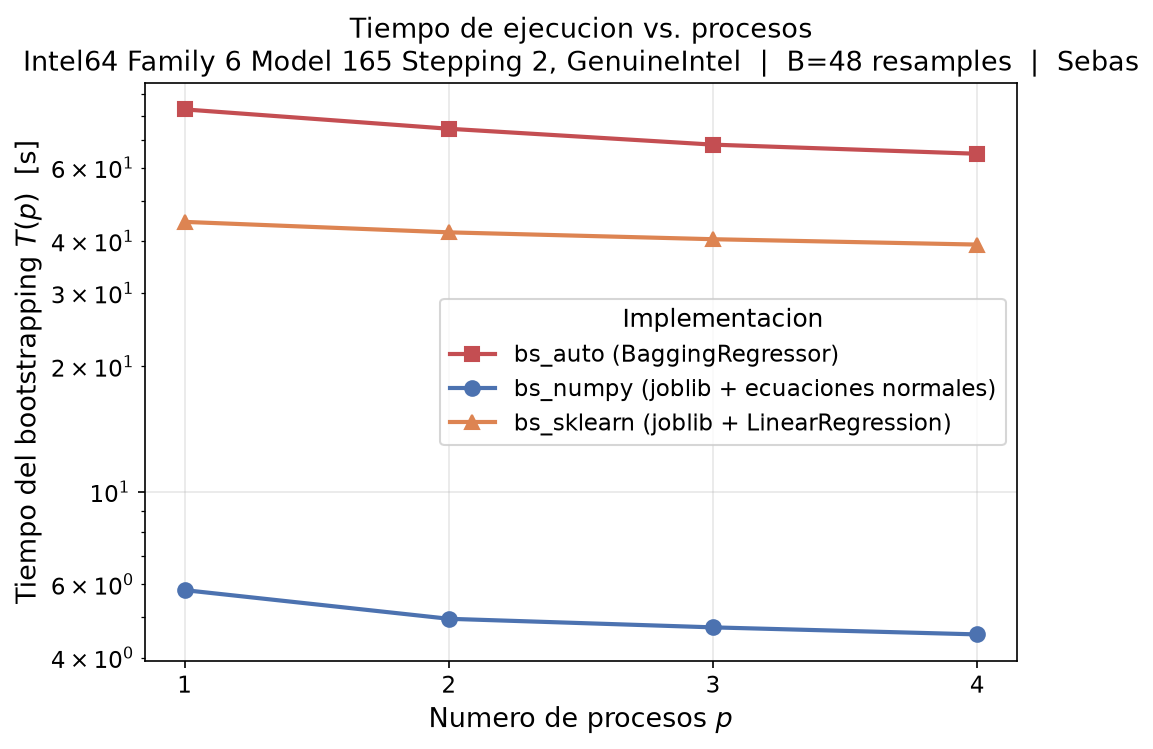
\includegraphics[width=0.75\textwidth]{results/tiempo_vs_p_sebas.png}\\
Gr\'afico tiempo vs. p (PC-1)
\end{center}

\begin{center}
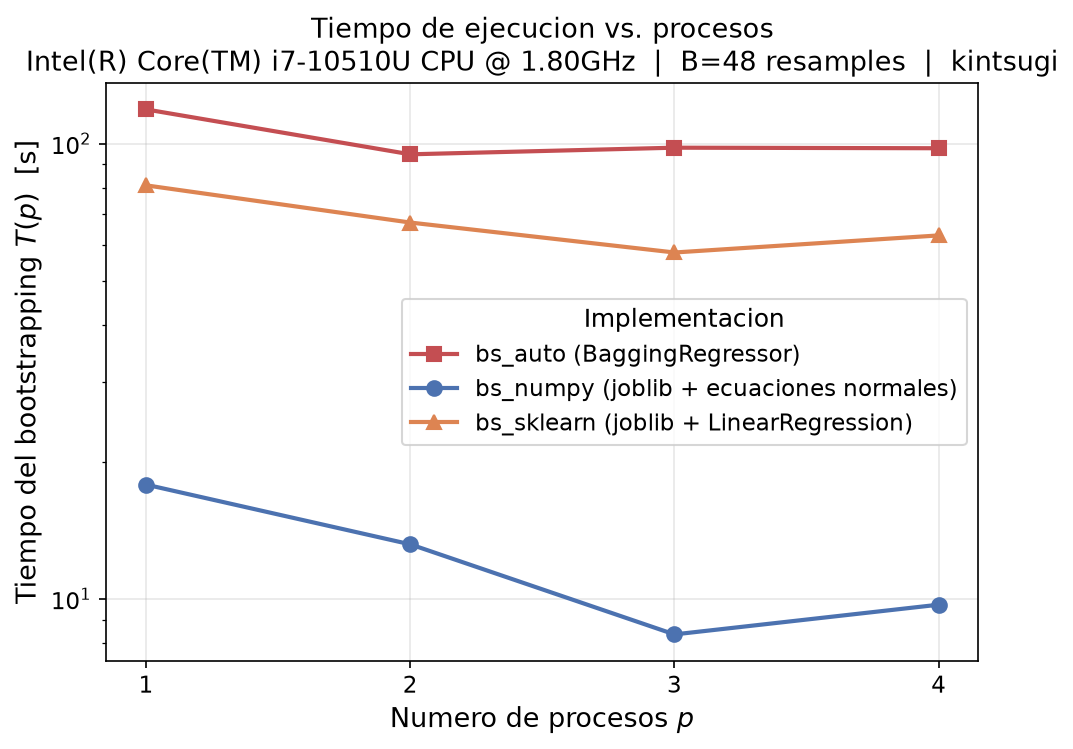
\includegraphics[width=0.75\textwidth]{results/tiempo_vs_p_kintsugi.png}\\
Gr\'afico tiempo vs. p (PC-2)
\end{center}

\begin{center}
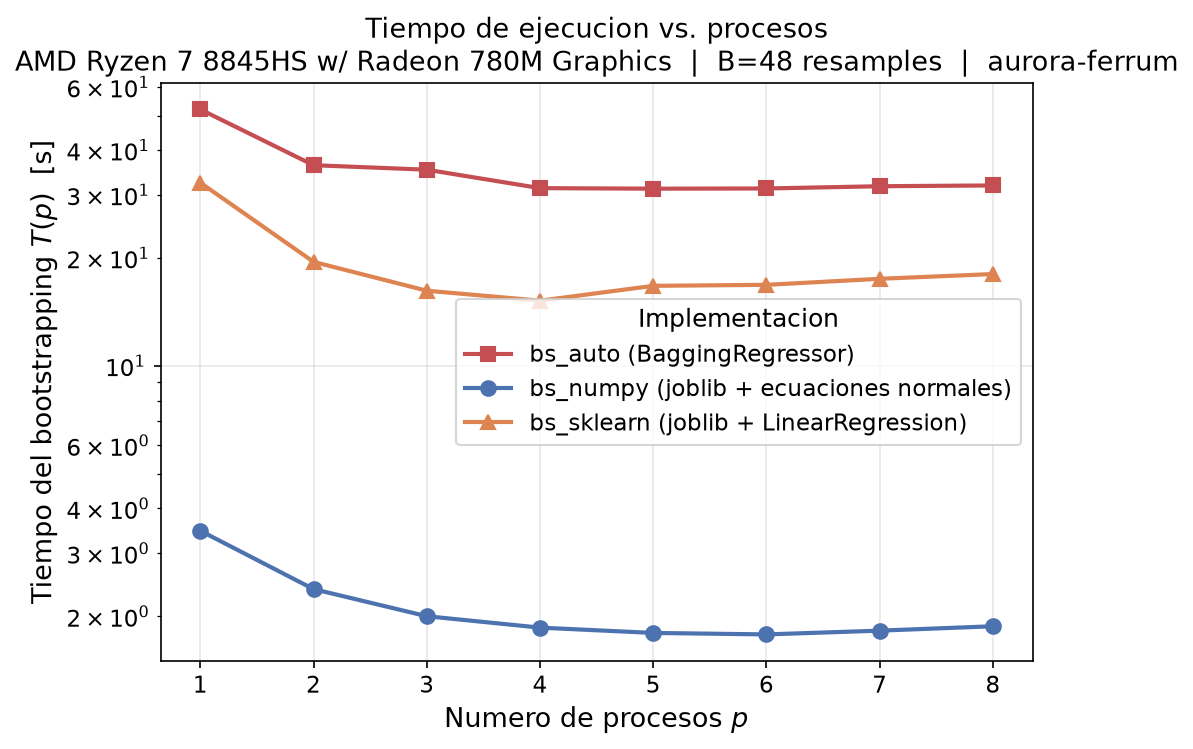
\includegraphics[width=0.75\textwidth]{results/tiempo_vs_p_aurora-ferrum.png}\\
Gr\'afico tiempo vs. p (PC-3)
\end{center}

\subsection*{g) T(p), S(p), E(p)}

\subsubsection*{PC-1}
\begin{center}
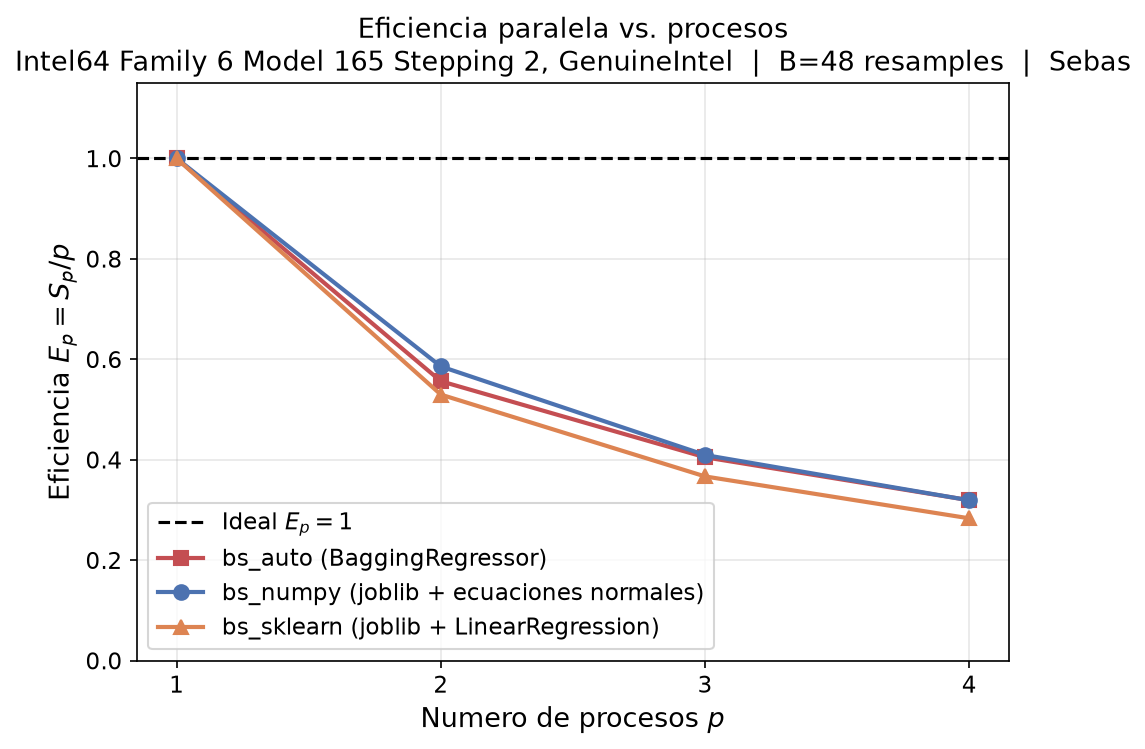
\includegraphics[width=0.75\textwidth]{results/eficiencia_sebas.png}\\
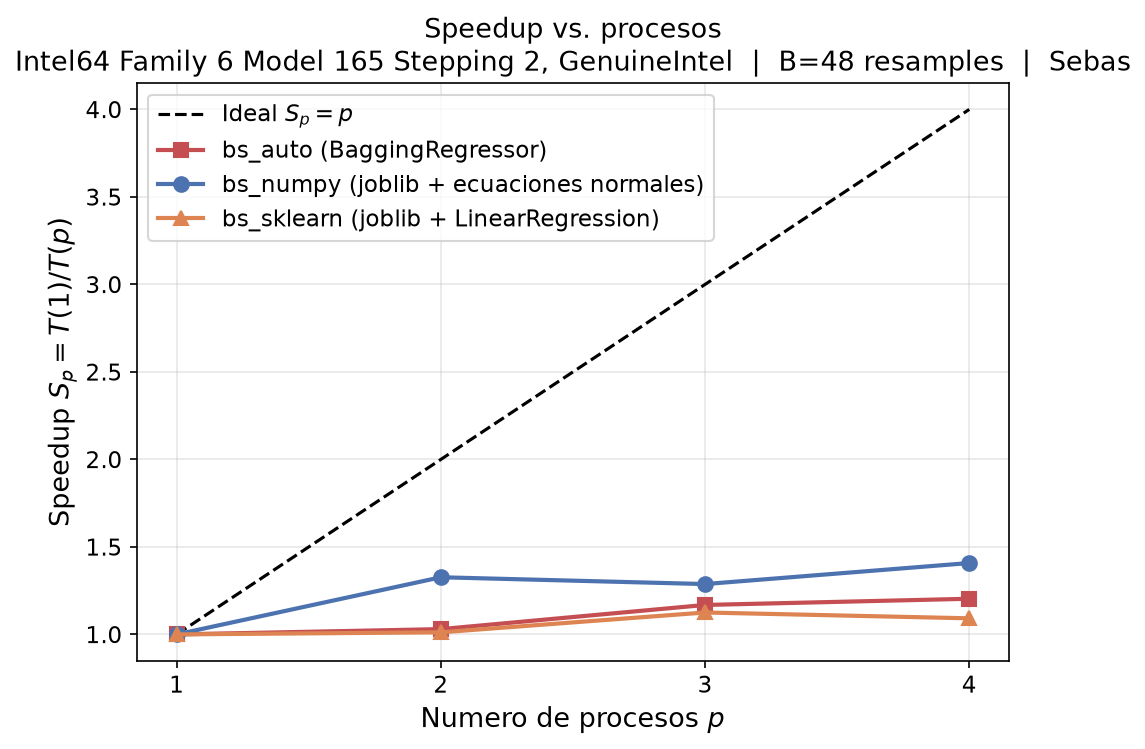
\includegraphics[width=0.75\textwidth]{results/speedup_sebas.png}
\end{center}

\subsubsection*{PC-2}
\begin{center}
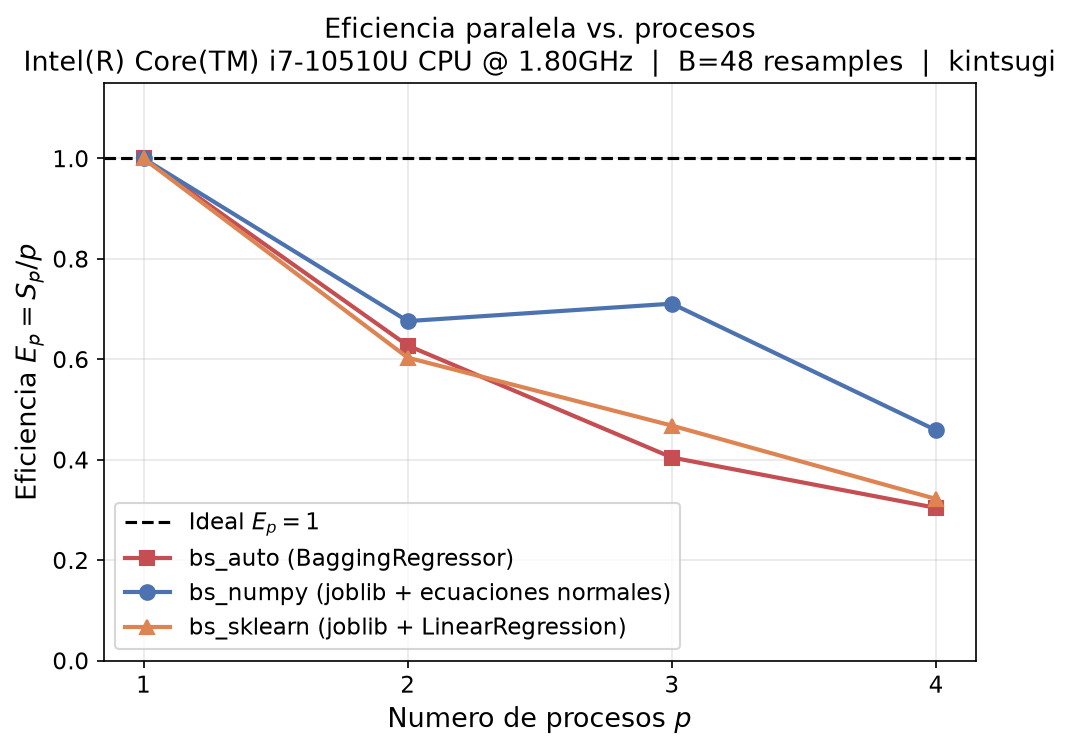
\includegraphics[width=0.75\textwidth]{results/eficiencia_kintsugi.png}\\
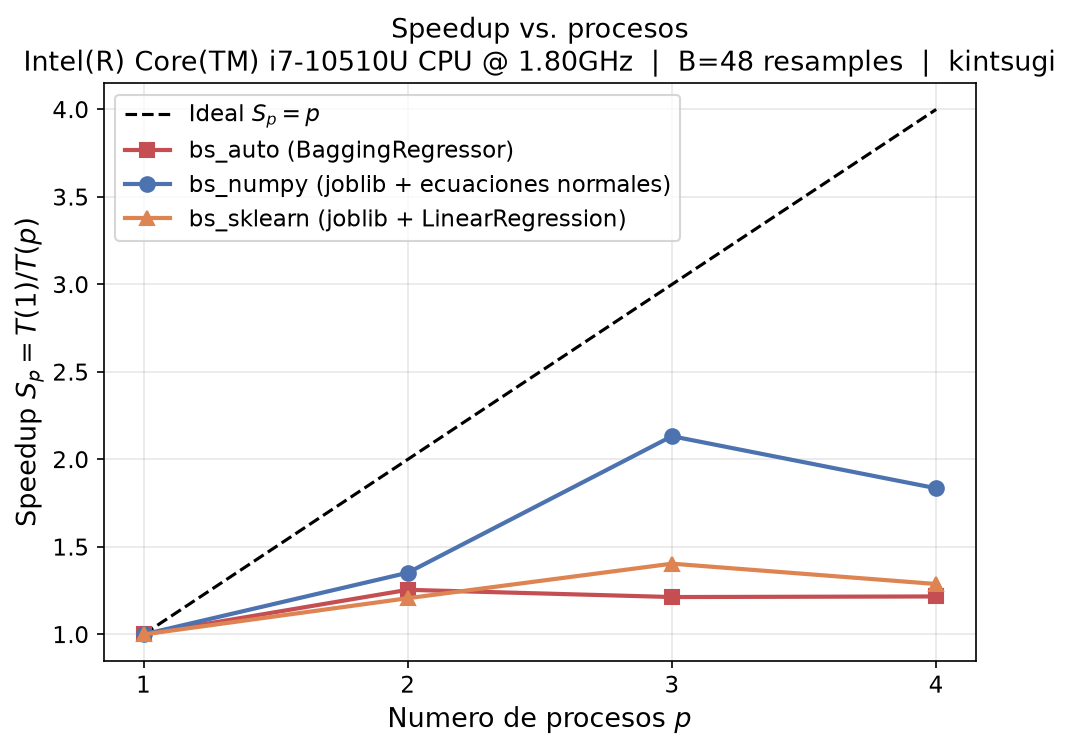
\includegraphics[width=0.75\textwidth]{results/speedup_kintsugi.png}
\end{center}

\subsubsection*{PC-3}
\begin{center}
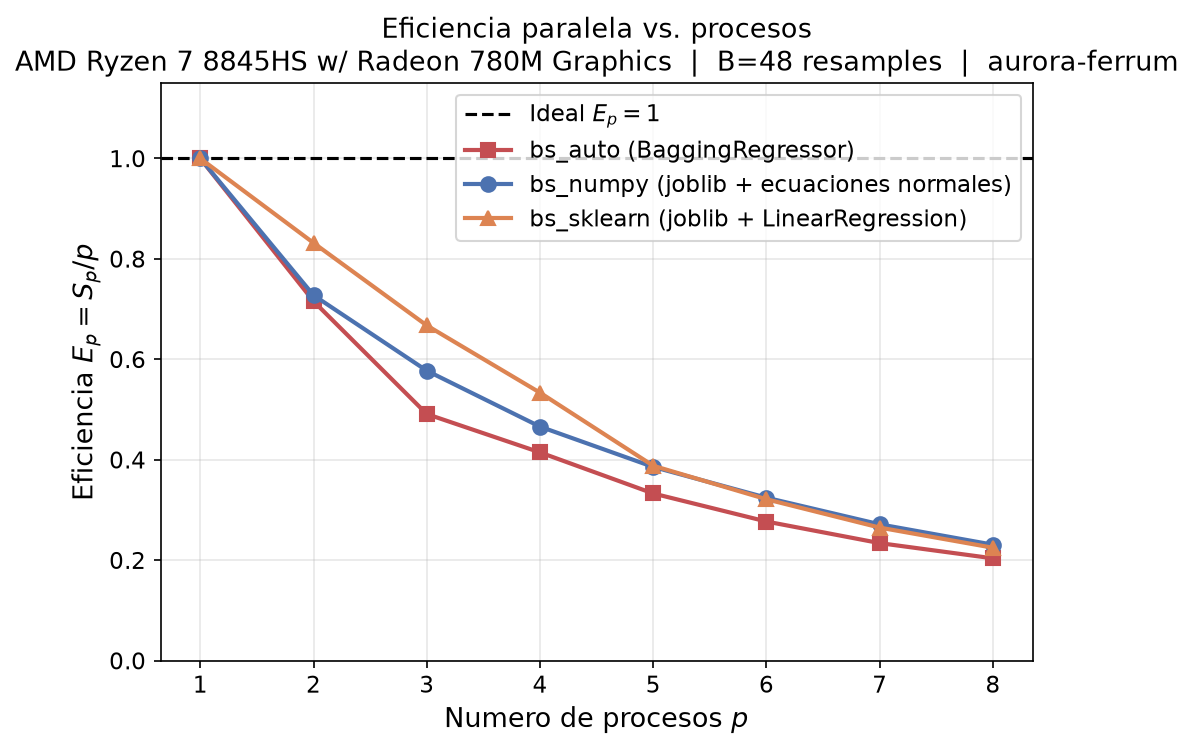
\includegraphics[width=0.75\textwidth]{results/eficiencia_aurora-ferrum.png}\\
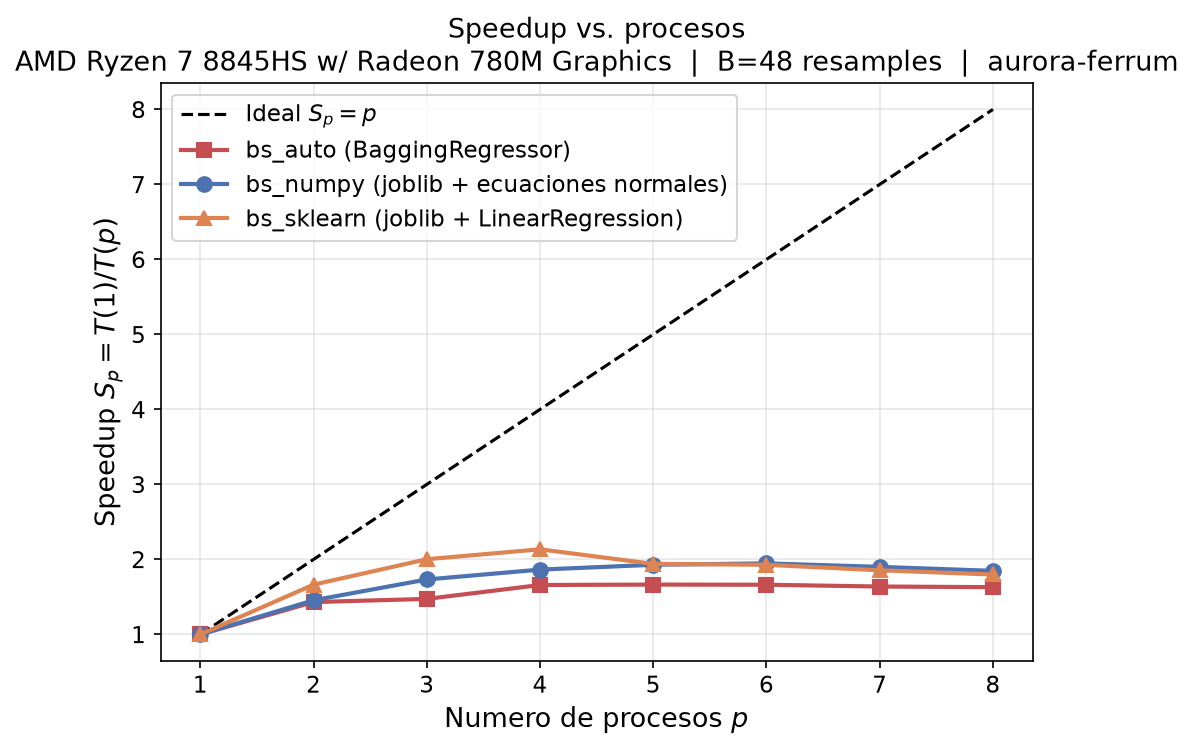
\includegraphics[width=0.75\textwidth]{results/speedup_aurora-ferrum.png}
\end{center}

\subsubsection*{bs\_auto}
\begin{center}
\begin{tabular}{clrrr}
\toprule
PC & p & T(p) [s] & S(p) & E(p) \\
\midrule
\multirow{4}{*}{PC-1} & 1 & 73.493 & 1.000 & 100.0\% \\
 & 2 & 71.334 & 1.030 & 51.5\% \\
 & 3 & 62.907 & 1.168 & 38.9\% \\
 & 4 & 61.056 & 1.204 & 30.1\% \\
\midrule
\multirow{4}{*}{PC-2} & 1 & 118.865 & 1.000 & 100.0\% \\
 & 2 & 94.721 & 1.255 & 62.7\% \\
 & 3 & 97.950 & 1.214 & 40.5\% \\
 & 4 & 97.677 & 1.217 & 30.4\% \\
\midrule
\multirow{8}{*}{PC-3} & 1 & 52.009 & 1.000 & 100.0\% \\
 & 2 & 36.338 & 1.431 & 71.6\% \\
 & 3 & 35.300 & 1.473 & 49.1\% \\
 & 4 & 31.354 & 1.659 & 41.5\% \\
 & 5 & 31.247 & 1.664 & 33.3\% \\
 & 6 & 31.287 & 1.662 & 27.7\% \\
 & 7 & 31.742 & 1.638 & 23.4\% \\
 & 8 & 31.904 & 1.630 & 20.4\% \\
\bottomrule
\end{tabular}
\end{center}

\subsubsection*{bs\_numpy}
\begin{center}
\begin{tabular}{clrrr}
\toprule
PC & p & T(p) [s] & S(p) & E(p) \\
\midrule
\multirow{4}{*}{PC-1} & 1 & 6.431 & 1.000 & 100.0\% \\
 & 2 & 4.848 & 1.327 & 66.3\% \\
 & 3 & 4.994 & 1.288 & 42.9\% \\
 & 4 & 4.568 & 1.408 & 35.2\% \\
\midrule
\multirow{4}{*}{PC-2} & 1 & 17.831 & 1.000 & 100.0\% \\
 & 2 & 13.185 & 1.352 & 67.6\% \\
 & 3 & 8.361 & 2.133 & 71.1\% \\
 & 4 & 9.716 & 1.835 & 45.9\% \\
\midrule
\multirow{8}{*}{PC-3} & 1 & 3.467 & 1.000 & 100.0\% \\
 & 2 & 2.382 & 1.455 & 72.8\% \\
 & 3 & 2.001 & 1.733 & 57.8\% \\
 & 4 & 1.860 & 1.864 & 46.6\% \\
 & 5 & 1.798 & 1.928 & 38.6\% \\
 & 6 & 1.781 & 1.947 & 32.4\% \\
 & 7 & 1.824 & 1.901 & 27.2\% \\
 & 8 & 1.876 & 1.848 & 23.1\% \\
\bottomrule
\end{tabular}
\end{center}

\subsubsection*{bs\_sklearn}
\begin{center}
\begin{tabular}{clrrr}
\toprule
PC & p & T(p) [s] & S(p) & E(p) \\
\midrule
\multirow{4}{*}{PC-1} & 1 & 42.273 & 1.000 & 100.0\% \\
 & 2 & 41.773 & 1.012 & 50.6\% \\
 & 3 & 37.568 & 1.125 & 37.5\% \\
 & 4 & 38.712 & 1.092 & 27.3\% \\
\midrule
\multirow{4}{*}{PC-2} & 1 & 80.963 & 1.000 & 100.0\% \\
 & 2 & 67.087 & 1.207 & 60.3\% \\
 & 3 & 57.659 & 1.404 & 46.8\% \\
 & 4 & 62.858 & 1.288 & 32.2\% \\
\midrule
\multirow{8}{*}{PC-3} & 1 & 32.474 & 1.000 & 100.0\% \\
 & 2 & 19.520 & 1.664 & 83.2\% \\
 & 3 & 16.216 & 2.003 & 66.8\% \\
 & 4 & 15.214 & 2.134 & 53.4\% \\
 & 5 & 16.734 & 1.941 & 38.8\% \\
 & 6 & 16.841 & 1.928 & 32.1\% \\
 & 7 & 17.509 & 1.855 & 26.5\% \\
 & 8 & 18.050 & 1.799 & 22.5\% \\
\bottomrule
\end{tabular}
\end{center}

\subsubsection*{Comentarios}

Se utiliz\'o T(1) como el tiempo con un s\'olo worker para par cada implementaci\'on en cada computador de forma que sea m\'as f\'acil comparar la p\'erdida de eficiencia.

\subsection*{h) Overhead seg\'un p}

\subsubsection*{bs\_auto}

$T_1$: PC-1 = 73.493 s, PC-2 = 118.865 s, PC-3 = 52.009 s

\begin{center}
\begin{tabular}{clrr}
\toprule
PC & p & T(p) [s] & T0(p) [s] \\
\midrule
\multirow{4}{*}{PC-1} & 1 & 73.493 & 0.000 \\
 & 2 & 71.334 & 69.175 \\
 & 3 & 62.907 & 115.228 \\
 & 4 & 61.056 & 170.731 \\
\midrule
\multirow{4}{*}{PC-2} & 1 & 118.865 & 0.000 \\
 & 2 & 94.721 & 70.577 \\
 & 3 & 97.950 & 174.985 \\
 & 4 & 97.677 & 271.843 \\
\midrule
\multirow{8}{*}{PC-3} & 1 & 52.009 & 0.000 \\
 & 2 & 36.338 & 20.667 \\
 & 3 & 35.300 & 53.891 \\
 & 4 & 31.354 & 73.407 \\
 & 5 & 31.247 & 104.226 \\
 & 6 & 31.287 & 135.713 \\
 & 7 & 31.742 & 170.185 \\
 & 8 & 31.904 & 203.223 \\
\bottomrule
\end{tabular}
\end{center}

\subsubsection*{bs\_numpy}

$T_1$: PC-1 = 6.431 s, PC-2 = 17.831 s, PC-3 = 3.467 s

\begin{center}
\begin{tabular}{clrr}
\toprule
PC & p & T(p) [s] & T0(p) [s] \\
\midrule
\multirow{4}{*}{PC-1} & 1 & 6.431 & 0.000 \\
 & 2 & 4.848 & 3.265 \\
 & 3 & 4.994 & 8.551 \\
 & 4 & 4.568 & 11.841 \\
\midrule
\multirow{4}{*}{PC-2} & 1 & 17.831 & 0.000 \\
 & 2 & 13.185 & 8.539 \\
 & 3 & 8.361 & 7.252 \\
 & 4 & 9.716 & 21.033 \\
\midrule
\multirow{8}{*}{PC-3} & 1 & 3.467 & 0.000 \\
 & 2 & 2.382 & 1.297 \\
 & 3 & 2.001 & 2.536 \\
 & 4 & 1.860 & 3.973 \\
 & 5 & 1.798 & 5.523 \\
 & 6 & 1.781 & 7.219 \\
 & 7 & 1.824 & 9.301 \\
 & 8 & 1.876 & 11.541 \\
\bottomrule
\end{tabular}
\end{center}

\subsubsection*{bs\_sklearn}

$T_1$: PC-1 = 42.273 s, PC-2 = 80.963 s, PC-3 = 32.474 s

\begin{center}
\begin{tabular}{clrr}
\toprule
PC & p & T(p) [s] & T0(p) [s] \\
\midrule
\multirow{4}{*}{PC-1} & 1 & 42.273 & 0.000 \\
 & 2 & 41.773 & 41.273 \\
 & 3 & 37.568 & 70.431 \\
 & 4 & 38.712 & 112.575 \\
\midrule
\multirow{4}{*}{PC-2} & 1 & 80.963 & 0.000 \\
 & 2 & 67.087 & 53.211 \\
 & 3 & 57.659 & 92.014 \\
 & 4 & 62.858 & 170.469 \\
\midrule
\multirow{8}{*}{PC-3} & 1 & 32.474 & 0.000 \\
 & 2 & 19.520 & 6.566 \\
 & 3 & 16.216 & 16.174 \\
 & 4 & 15.214 & 28.382 \\
 & 5 & 16.734 & 51.196 \\
 & 6 & 16.841 & 68.572 \\
 & 7 & 17.509 & 90.089 \\
 & 8 & 18.050 & 111.926 \\
\bottomrule
\end{tabular}
\end{center}

\subsubsection*{Comentarios}

Notamos que existe un overhead que creciente con el n\'umero de procesos. Que se correlaciona con el costo de realizar un fork y copiar los datos del proceso dado que estos no comparten memoria a diferencia de los threads.

\subsection*{i) Versi\'on m\'as eficiente}

Notamos que la versi\'on m\'as eficiente fue por lejos la implementaci\'on de numpy. Como se vi\'o en los datos expuestos anteriormente, el desempe\~no fue el mejor en los 3 equipos probados. Obteniendo el menor tiempo, y mayor retenci\'on de eficiencia y speedup a medida que se agregan workers.

\subsubsection*{PC-3 (aurora-ferrum, p\_max=8)}

\begin{center}
\begin{tabular}{rrrrrr}
\toprule
p & t (inner threads) & tiempo bootstrap [s] & ancho IC medio & cobertura beta* & $\|$mean(b)-bhat$\|$ \\
\midrule
1 & 1 & 5.348 & 0.011812 & 0.950 & 4.29e-04 \\
1 & 2 & 4.281 & 0.011812 & 0.950 & 4.29e-04 \\
1 & 3 & 4.082 & 0.011812 & 0.950 & 4.29e-04 \\
1 & 4 & 4.440 & 0.011812 & 0.950 & 4.29e-04 \\
1 & 5 & 5.908 & 0.011812 & 0.950 & 4.29e-04 \\
1 & 6 & 3.895 & 0.011812 & 0.950 & 4.29e-04 \\
1 & 7 & 5.978 & 0.011812 & 0.950 & 4.29e-04 \\
1 & 8 & 6.485 & 0.011812 & 0.950 & 4.29e-04 \\
2 & 1 & 3.486 & 0.011812 & 0.950 & 4.29e-04 \\
2 & 2 & 3.041 & 0.011812 & 0.950 & 4.29e-04 \\
2 & 3 & 2.895 & 0.011812 & 0.950 & 4.29e-04 \\
2 & 4 & 3.044 & 0.011812 & 0.950 & 4.29e-04 \\
3 & 1 & 2.355 & 0.011812 & 0.950 & 4.29e-04 \\
3 & 2 & 2.260 & 0.011812 & 0.950 & 4.29e-04 \\
4 & 1 & 2.657 & 0.011812 & 0.950 & 4.29e-04 \\
4 & 2 & 3.013 & 0.011812 & 0.950 & 4.29e-04 \\
5 & 1 & 2.534 & 0.011812 & 0.950 & 4.29e-04 \\
6 & 1 & 2.350 & 0.011812 & 0.950 & 4.29e-04 \\
7 & 1 & 2.361 & 0.011812 & 0.950 & 4.29e-04 \\
8 & 1 & 2.158 & 0.011812 & 0.950 & 4.29e-04 \\
\bottomrule
\end{tabular}
\end{center}

\subsubsection*{PC-1 (sebas, p\_max=4)}

\begin{center}
\begin{tabular}{rrrrrr}
\toprule
p & t (inner threads) & tiempo bootstrap [s] & ancho IC medio & cobertura beta* & $\|$mean(b)-bhat$\|$ \\
\midrule
1 & 1 & 11.195 & 0.011812 & 0.950 & 4.29e-04 \\
1 & 2 & 8.553 & 0.011812 & 0.950 & 4.29e-04 \\
1 & 3 & 16.773 & 0.011812 & 0.950 & 4.29e-04 \\
1 & 4 & 15.453 & 0.011812 & 0.950 & 4.29e-04 \\
2 & 1 & 6.443 & 0.011812 & 0.950 & 4.29e-04 \\
2 & 2 & 6.368 & 0.011812 & 0.950 & 4.29e-04 \\
3 & 1 & 5.476 & 0.011812 & 0.950 & 4.29e-04 \\
4 & 1 & 5.361 & 0.011812 & 0.950 & 4.29e-04 \\
\bottomrule
\end{tabular}
\end{center}

\subsection*{j) Comparaci\'on de resultados}

Notamos que los mejores resultados se alcanzaron con un \'unico thread, con un numero de procesos igual al n\'umero de nucleos f\'isicos de cada m\'aquina. Cabe mencionar tambi\'en que incluso bajo los mismos valores de p,t. PC-3 tuvo un mejor desempe\~no. Probablemente debido a la diferencia de frecuenica de los procesadores, haciendo la ejecuci\'on de PC-3 m\'as r\'apida. Esto resalta la importancia de comparar cada m\'aquina por separado, dado que estas diferencias de performance influyen tanto en el tiempo de ejecuci\'on m\'inimo, como tambi\'en determinan la combinaci\'on \'optima de threads/procesos en cada caso.

\section*{Uso de IA}

Se utiliz\'o IA para:
\begin{itemize}
  \item Buscar posibles optimizaciones al c\'odigo implementado iterativamente (Claude)
  \item Debuggear errores de c\'odigo (Claude)
  \item Explicar detalles de implementaci\'on de las libererias que impactaban en el c\'odigo y sus resultados (Claude)
  \item Generar un script de bash que pruebe todas las combinaciones relevantes de p,t dado un valor de p\_max (Claude)
  \item Generar tablas de markdown a partir de logs de ejecuci\'on (ChatGPT)
  \item Generar un archivo de latex compilable a partir de un archivo de markdown (ChatGPT)
\end{itemize}

\end{document}
